%   Config file:    RTKLIB, EKF
%    IMC:            gnssData, estimatedStateEKF, externalEstimatedState
    
%    RTKLIB task:    Playback file, serial read, apply corrections, dispatch observables
%    EKF:            Tightly coupled, extended kalman filter, PV-estimation (PVA?)
For the system running on hardware, two DUNE tasks have been implemented. One task interfaces the RTKLIB code base, while the other implements the EKF described in section \ref{sec:imp:ekf}. Additionally, several preimplemented DUNE tasks are included in the full system. Most notably, an Ardupilot task for connecting DUNE and Ardupilot, and a logging task for storing IMU messages. The Ardupilot task is necessary for two reasons. Firstly, it provides the system with IMU measurements from the Pixhawk IMU and, secondly, it estimates and dispatches the vehicle attitude, which is unmodeled in the EKF. The logging task is necessary for testing, as mentioned in section \ref{sec:imp:testing}. A block diagram of the system is shown in figure \ref{fig:dune-tasks}.\\

    \begin{figure}[!htbp]
    \centering
    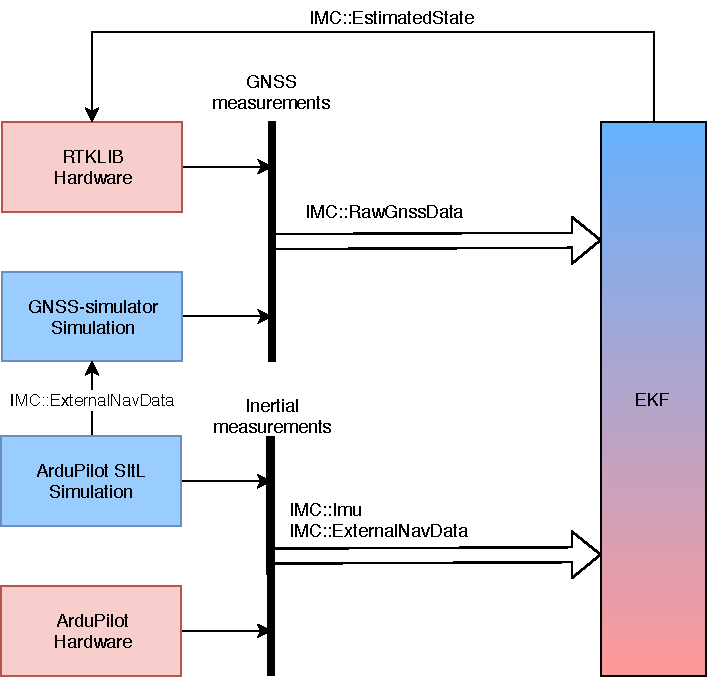
\includegraphics[scale=0.8]{Implementation/Images/dune-tasks.pdf}
    \caption{Overview of the EKF and the tasks it communicates with. Each box is a distinct task. The tasks are color coded as follows; The blue boxes are tasks used for the simulator (section \ref{sec:imp:simulator}), while the red ones run on hardware. The EKF task depends only on the IMC-messages and runs regardless of either profile.}
    \label{fig:dune-tasks}
    \end{figure}

\subsection{RTKLIB interface}
    %Based on the rtkrcv commandline program from rtklib
    %Handles rtklib config and cmd files
    %Can play back log files as mentioned in section \ref{sec:imp:simulators}
    %Unwanted features of rtkrcv. State estimation, terminal, sat stats, stream stats
    The main purpose of the RTKLIB task is to read GNSS measurements from a stream and dispatch these on the IMC bus. It is based on the RTKLIB commandline program rtkrcv, and keeps much of the same functionality, with a few notable exceptions. The task is configured through a configuration file, also called a conf file, and can configure a connected serial device based on receiver configuration file, also called a CMD file. Measurements can be read from different sources, such as log files or serial devices, and, if specified in the conf file, they can be logged in different file formats as well. Unlike the rtkrcv program however, the task does not estimate any state variables, it does not run separately in a terminal and can not output any kind of status screens.\\
    
    The RTKLIB code base can be accessed in DUNE by adding it as a third party vendor library. However, RTKLIB builds its programs with makefiles only, while DUNE relies on CMake. Therefore, a CMake file is added to the vendor, based on the makefile for rtkrcv. To enable multi-GNSS functionality a flag must be set for each enabled constellation. However, this changes the value of several internal preprocessor macros, which in turn is used to set the size of RTKLIB's internal storage structs. To avoid memory errors it is therefore necessary that all DUNE tasks working with RTKLIB structs add the same flags to their own CMake files.\\
    
    \begin{table}[!htbp]
    \centering
    \begin{tabularx}{\textwidth}{ |l|X| }\hline
        \textbf{Message name}   & \textbf{Message members}  \\\hline
        RawGNSSdata & 
        \begin{minipage}[t]{0.7\textwidth}
            \begin{itemize}
                \item Measurement time (GPS week and time)
                \item Satellite observables (List of IMC message)
            \end{itemize}
        \end{minipage}\\\hline
        RawGNSSsatObs &
        \begin{minipage}[t]{0.7\textwidth}
            \begin{itemize}
                \item GNSS constellation ID
                \item Pseudo-range, doppler-shift and carrier phase
                \item Satellite position and velocity
                \item Measurement standard deviations
            \end{itemize}
        \end{minipage}\\\hline
    \end{tabularx}
    \caption{GNSS IMC messages and relevant members}
    \label{tab:imc-gnss}
    \end{table}
    
    After configuration files have been read and storage structs have been allocated, the task enters its main execution loop. This reads data from the input stream, which will eventually store an ephemeris. For each available ephemeris, satellite position and velocity is calculated. Measurements are then collected, corrected for atmospheric, sagnac and satellite clock errors and finally dispatched, with satellite position and velocity, as a RawGNSSdata IMC message, shown in table \ref{tab:imc-gnss}. The corrections are a function of the receiver position, which the RTKLIB task receives by binding the EstimatedState IMC message, which in this implementation is dispatched from the EKF. If set in the configuration file, the task stores both measurements and receiver position in a UBX and a POS file, respectively, each iteration. Note that the name \textit{RawGNSSdata} is somewhat misleading, as corrections have been applied to the measurements. This IMC message type is simply used because it was implemented prior to this thesis and readily available.
    
\subsection{Extended Kalman filter}
    \label{sec:imp:ekf-dune}
    This task estimates position, velocity, receiver clock bias and receiver clock bias rate based on acceleration and GNSS measurements. It implements the filter described in section \ref{sec:imp:ekf}. The measurements are received from the IMU and RawGNSSdata messages, attitude comes from ExternalNavData and finally position and velocity is output in the EstimatedState message as seen in tables \ref{tab:imc-gnss} and \ref{tab:imc-filter}.\\
    
    \begin{table}[!htbp]
    \centering
    \begin{tabularx}{\textwidth}{ |l|X| }\hline
        \textbf{Message name}   & \textbf{Message members}  \\\hline
        EstimatedState & 
        \begin{minipage}[t]{0.7\textwidth}
            \begin{itemize}
                \item Vehicle position (longitude, latitude, height)
                \item Vehicle attitude (between body and NED)
                \item Vehicle velocity (of body, with respect to NED)
            \end{itemize}
        \end{minipage}\\\hline
        ExternalNavData & 
        \begin{minipage}[t]{0.7\textwidth}
            \begin{itemize}
                \item Estimated state (IMC message)
                \item Nav Data Type (Status of estimated state)
            \end{itemize}
        \end{minipage}\\\hline
        Imu &
        \begin{minipage}[t]{0.7\textwidth}
            \begin{itemize}
                \item Acceleration (IMC message)
                \item AngularVelocity (IMC message)
            \end{itemize}
        \end{minipage}\\\hline
        Acceleration & 
        \begin{minipage}[t]{0.7\textwidth}
            \begin{itemize}
                \item Device time
                \item X, Y and Z acceleration components
            \end{itemize}
        \end{minipage}\\\hline
        AngularVelocity & 
        \begin{minipage}[t]{0.7\textwidth}
            \begin{itemize}
                \item Device time
                \item X, Y and Z angular velocity components
            \end{itemize}
        \end{minipage}\\\hline
    \end{tabularx}
    \caption{Imu and State IMC messages with relevant members}
    \label{tab:imc-filter}
    \end{table}
    %Describe each consume
    %Describe timestep
    %Describe numeric van loan?
    %GNSS
    Each time a set of GNSS measurements are received, they run the measurement step of the EKF. The rate of the measurements depend on how the receiver is configured, and has been set to 10 Hz in this thesis. Similarily, each IMU measurement runs the prediction step. To sufficiently capture the dynamics of the system, these measurements arrive at a higher frequency than the GNSS measurements, at about 30 Hz, although this can vary. As each prediction step discretizes the system, the timestep between measurements should be as exact as possible, and a timestamp is therefore added to each measurement.\\ \todo{30 Hz is very low}
    
    %ExternalNavData
    A separate state estimate is received from the ArduPilot task in the ExternalNavData message. Although only the attitude is used during normal operation, the whole state is kept for both redundancy, and to have a reference during testing and tuning. The external state estimate represents position by latitude, longitude and height, while the attitude denotes the rotation between the body and NED frame. However, as the EKF works with the ECEF frame of reference, this state estimate must be transformed to the ECEF frame as well. The rotation matrix from the body frame to the ECEF frame is calculated as follows
    \begin{equation}
        \mathbf{R}^e_b = \mathbf{R}^e_n\mathbf{R}^n_b
    \end{equation}
    where the matrices on the right hand side are the rotation matrix from the NED frame to the ECEF frame and from the body frame to the NED frame. The first is calculated from latitude and longitude by equation \ref{eq:Ren}, while the second comes from equation \ref{eq:Rnb-eul}, from appendix \ref{app:roten}. Equations \ref{eq:pred-pos} and \ref{eq:pred-vel} assumes the gravitational vector in the ECEF frame to be known, which is found by rotating the vector defined by \ref{def:gn}. 
    
    
    \todo{Mention sourcetrail?}
    \todo{Logs matrices}
    